\documentclass[12pt]{article}
\usepackage[paperwidth=320mm,paperheight=180mm,margin=16mm,noheadfoot]{geometry}
\usepackage{lmodern,amsmath,graphicx,xcolor,booktabs}
\definecolor{ink}{HTML}{142B3A}
\definecolor{accent}{HTML}{216C70}
\definecolor{muted}{HTML}{526471}
\renewcommand{\familydefault}{\sfdefault}
\pagestyle{empty}
\raggedright
\setlength{\parindent}{0pt}
\setlength{\parskip}{9pt}
\newcommand{\slide}[2]{\newpage
  {\color{accent}\small\bfseries #1}\hfill{\color{muted}\small CSE 5403 \quad \thepage}\par
  \vspace{2mm}{\color{ink}\bfseries\fontsize{29}{34}\selectfont #2}\par\vspace{3mm}}
\newcommand{\lead}[1]{{\large\color{ink}#1}\par}
\newcommand{\metric}[2]{{\color{accent}\bfseries\fontsize{38}{43}\selectfont #1}\par
  {\color{muted}\large #2}\par}
\newcommand{\captionline}[1]{{\color{muted}\small #1}\par}
\begin{document}
\color{ink}

{\color{accent}\large\bfseries CSE 5403 \quad ALGORITHMS FOR NONLINEAR OPTIMIZATION}
\vspace{19mm}

{\bfseries\fontsize{43}{48}\selectfont Robust Multi-Position\\[2mm]Parametric Room Equalization}
\vspace{10mm}

\lead{One six-filter equalizer for multiple measured listening positions}
\lead{Projected generalized Gauss--Newton \enspace $\cdot$ \enspace MeshRIR spatial holdout}
\vfill
{\color{accent}\rule{0.24\linewidth}{2pt}}

\slide{RESEARCH QUESTION}{Can one equalizer help unseen listening positions?}
\vspace{4mm}
\begin{minipage}[t]{.51\linewidth}
\lead{A reflection or cancellation changes with microphone position.}
\lead{One global correction can move all responses closer to a target while preserving their pointwise spread.}
\lead{We compare single-seat, mean, and robust shared designs.}
\end{minipage}\hfill
\begin{minipage}[t]{.42\linewidth}
\vspace{0pt}
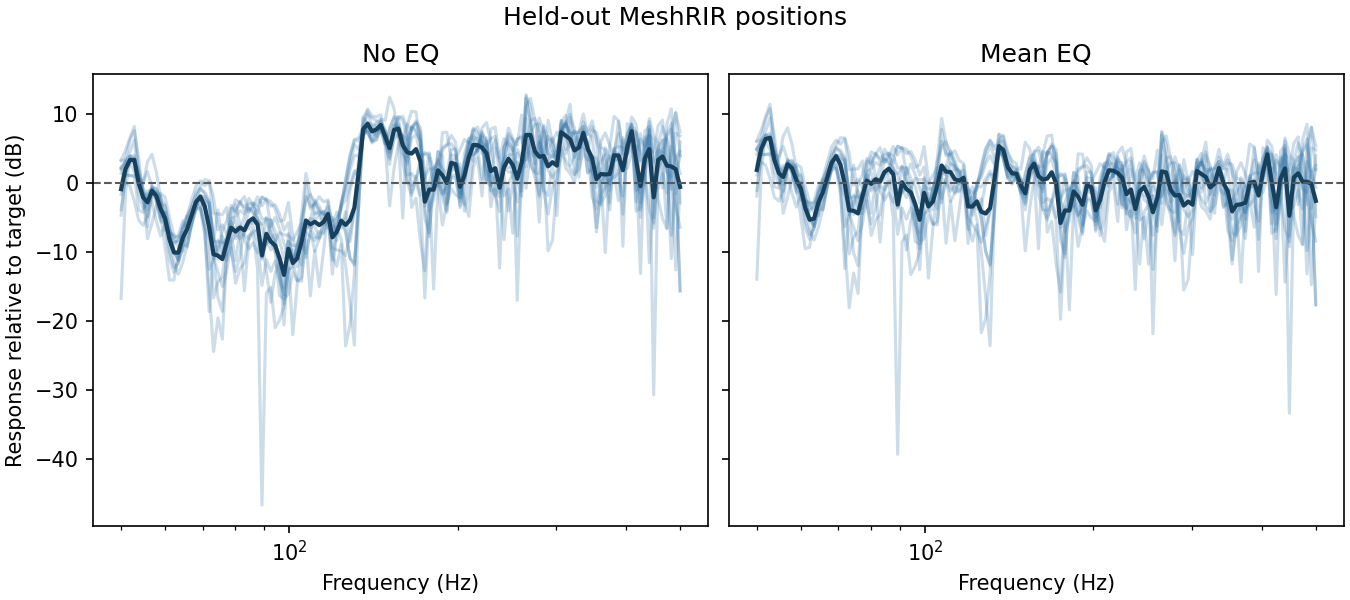
\includegraphics[width=\linewidth]{results/smoke/responses.png}
\captionline{Measured responses from the 12-position smoke holdout.}
\end{minipage}

\slide{MEASUREMENTS}{The main holdout is separated by 25 cm}
\begin{minipage}[t]{.39\linewidth}
\vspace{2mm}
\metric{126}{fixed held-out positions}
\lead{One source, middle MeshRIR plane, 5 cm measurement grid.}
\lead{Three repeats with 3, 10, or 20 nested training positions.}
\end{minipage}\hfill
\begin{minipage}[t]{.57\linewidth}
\vspace{0pt}
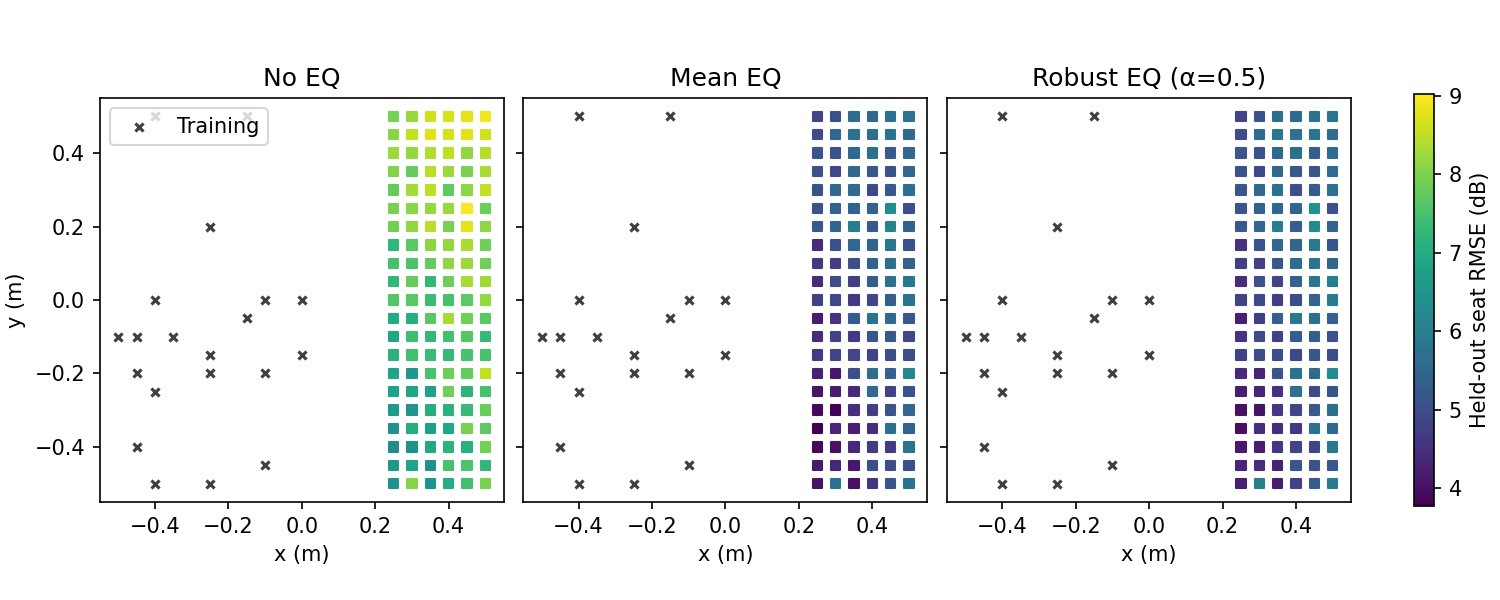
\includegraphics[width=\linewidth]{results/main/spatial_map.png}
\captionline{Crosses mark training locations. Colored squares show held-out RMSE on a shared scale.}
\end{minipage}

\slide{FORMULATION}{One correction, two loss terms}
\lead{Six peaking biquads, 18 parameters, and a 50--500 Hz fitting band.}
\[
 e_m=\tfrac12\sum_j w_j(h_{mj}+u_j(\theta)-T)^2
\]
\[
 F_{\alpha,\tau}=\alpha\,\overline e+
 (1-\alpha)\tau\log\!\left(M^{-1}\sum_m e^{e_m/\tau}\right)
 +\tfrac{\lambda}{2}\sum_k g_k^2 .
\]
\lead{The primary robust fit uses \(\alpha=0.5\) and \(\tau=2~\mathrm{dB}^2\).}
\lead{The bounds are \(-12\) to \(+6\) dB per filter and \(Q=0.3\) to \(10\). A combined boost diagnostic tracks headroom.}

\slide{ANALYTICAL BENCHMARK}{Spatial variance sets a mean-error floor}
\[
 \underbrace{M^{-1}\sum_m(h_{mj}+u_j-T)^2}_{\text{Mean squared error at frequency }j}
 =
 \underbrace{\operatorname{Var}_m(h_{mj})}_{\text{Spatial variance}}
 +
 \underbrace{(\overline h_j+u_j-T)^2}_{\text{Mean-response error}}
\]
\vspace{5mm}
\begin{minipage}[t]{.43\linewidth}
\metric{3.61 dB}{Unrestricted pooled RMSE floor}
\end{minipage}\hfill
\begin{minipage}[t]{.49\linewidth}
\metric{4.29 dB}{Best-training-objective L-BFGS-B mean fit}
\end{minipage}\par
\captionline{Training data from the nine-position matched solver benchmark.}

\slide{NONLINEAR OPTIMIZATION}{The solver keeps the worst-seat curvature}
\[
 B=J^\top J+\frac{1-\alpha}{\tau}\operatorname{Cov}_{p}(J^\top r_m)
       +\lambda\nabla^2 R .
\]
\vspace{2mm}
\begin{itemize}
\setlength\itemsep{10pt}
\item Use the common analytical Jacobian and a damped free-variable solve.
\item Project the trial step to the box and test descent after projection.
\item Fall back to a scaled projected gradient if the damped step fails.
\item Compare with L-BFGS-B on the same loss, starts, bounds, and projected-gradient tolerance.
\end{itemize}

\slide{SOLVER RESULTS}{Gauss--Newton used fewer calls}
\begin{minipage}[t]{.48\linewidth}
\vspace{0pt}
\begin{tabular}{lrr}
\toprule
Median evaluations & Mean & Robust\\
\midrule
Gauss--Newton & 116 & 129 \\
L-BFGS-B & 399 & 353 \\
\bottomrule
\end{tabular}
\vspace{4mm}

\lead{All 20 fits reached the shared stopping tolerance.}
\lead{L-BFGS-B found the lowest objective for both losses.}
\end{minipage}\hfill
\begin{minipage}[t]{.48\linewidth}
\vspace{0pt}
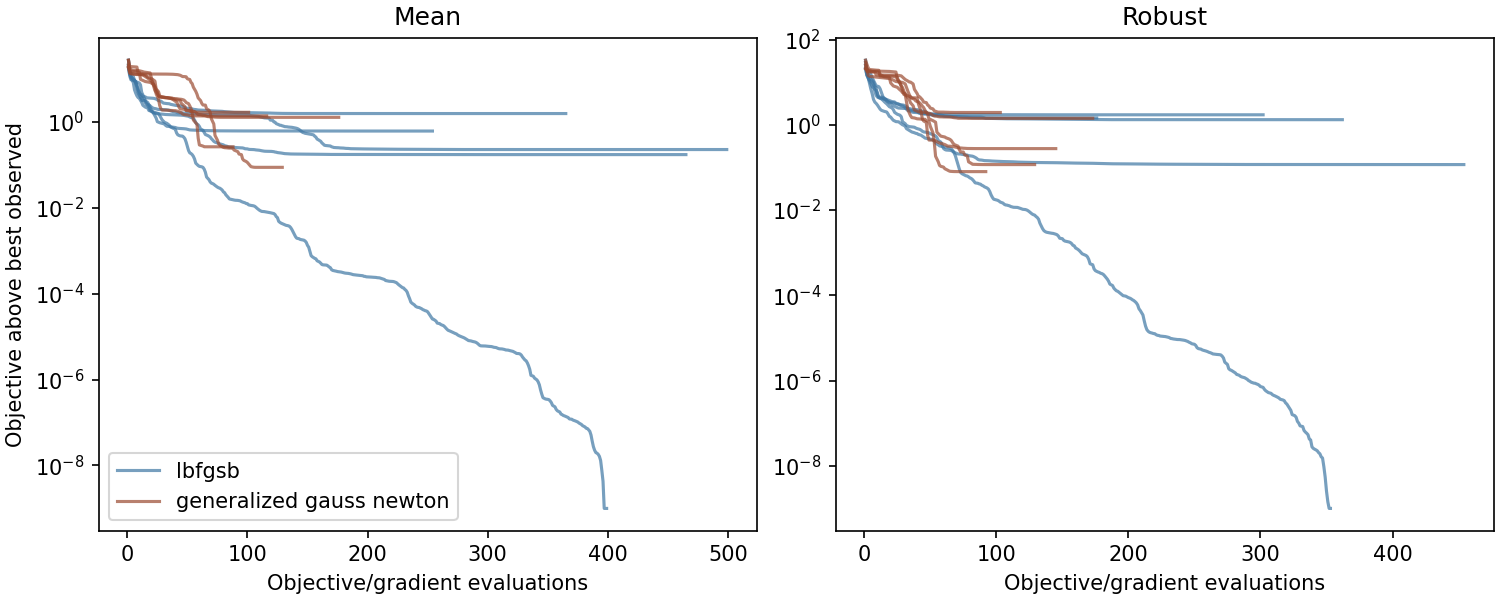
\includegraphics[width=\linewidth]{results/main/convergence.png}
\captionline{Objective above the best observed value within each loss.}
\end{minipage}

\slide{ACOUSTIC RESULTS}{Shared EQ reduced held-out error}
\vspace{4mm}
{\large
\begin{tabular}{lrr}
\toprule
Method & Pooled RMSE & Worst-seat RMSE\\
\midrule
No EQ & 7.73 dB & 9.02 dB \\
Single-seat EQ & 4.93 dB & 6.17 dB \\
Mean EQ & 5.10 dB & 6.32 dB \\
Robust EQ, \(\alpha=0.5\) & 5.13 dB & 6.36 dB \\
\bottomrule
\end{tabular}
}
\vspace{4mm}

\captionline{Median across three spatial training selections with 20 positions each.}
\lead{The center-seat fit was competitive on this particular held-out strip.}

\slide{SPATIAL GENERALIZATION}{The robust gain rarely transferred}
\begin{minipage}[t]{.37\linewidth}
\vspace{0pt}
\metric{7 of 9}{training comparisons favored robust EQ}
\vspace{3mm}
\metric{2 of 9}{holdout comparisons favored robust EQ}
\captionline{Median worst-seat differences were \(-0.036\) dB in training and \(+0.064\) dB on the holdout.}
\end{minipage}\hfill
\begin{minipage}[t]{.59\linewidth}
\vspace{0pt}
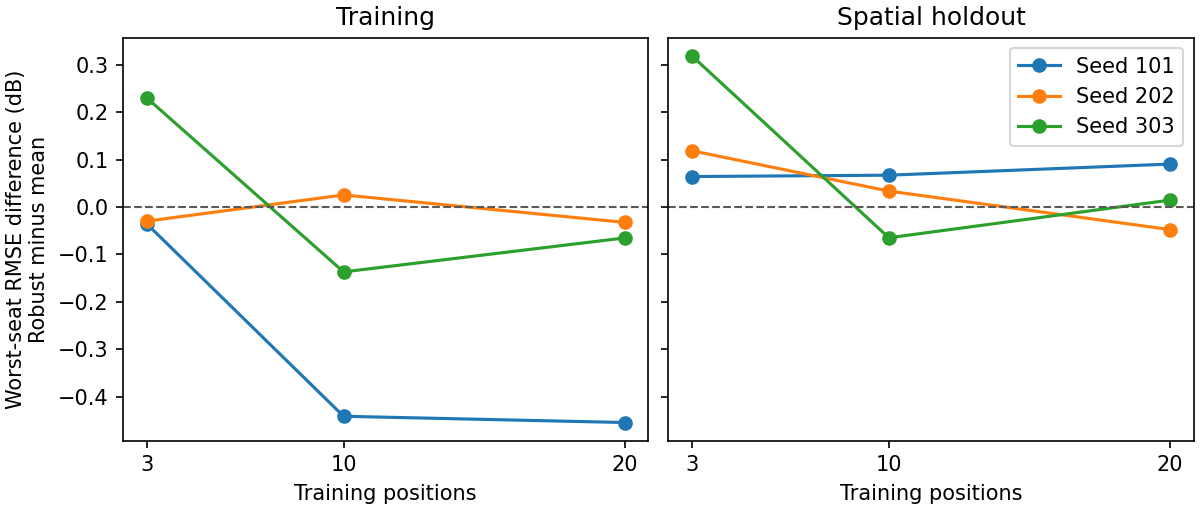
\includegraphics[width=\linewidth]{results/ablation/paired_worst_seat.png}
\captionline{Each line connects nested training counts from one seed. Negative differences favor robust EQ.}
\end{minipage}

\slide{TEMPERATURE ABLATION}{Continuation cost more calls on all five starts}
\lead{Training-only pilot selected \(32\rightarrow8\rightarrow2~\mathrm{dB}^2\).}
\vspace{2mm}
{\large
\begin{tabular}{lrr}
\toprule
Method & Median evaluations & Best final objective\\
\midrule
Direct & 129 & 10.995 \\
Continuation & 233 & 11.243 \\
\bottomrule
\end{tabular}
}
\vspace{4mm}

\lead{Continuation improved the paired final objective once. All ten endpoints met the same stationarity tolerance.}
\captionline{Both methods shared the final temperature, starts, and total evaluation cap.}

\slide{INITIALIZATION ABLATION}{Peak placement helped at the start}
\lead{The five seeded random-center starts used the same cut gains and \(Q\) values as the peak-informed start.}
\vspace{2mm}
\begin{minipage}[t]{.46\linewidth}
\metric{9 of 9}{lower starting objective than the split-level random median}
\end{minipage}
\begin{minipage}[t]{.49\linewidth}
\metric{4 of 9}{lower final objective than the split-level random median}
\end{minipage}
\vspace{3mm}

\lead{Peak placement used a median of 18 more calls per paired comparison. All 70 fits reached stationarity.}

\slide{CONCLUSIONS}{What the measured results support}
\begin{itemize}
\setlength\itemsep{10pt}
\item A common low-frequency EQ substantially reduced held-out error for this source and spatial block.
\item Structured curvature reduced calls to stationarity, and the lowest training objective depended on the solver and start.
\item The tested worst-seat objective and warm-start strategies showed limited benefit on their primary comparison metrics.
\item The experiment covers one room, one source, a 50--500 Hz magnitude band, and one fixed spatial holdout.
\end{itemize}
\captionline{Methods, references, and exact run records accompany the report. Data: MeshRIR S1-M3969, release 1.2, CC BY 4.0.}

\end{document}
